\chapter{Database Locking, Scanning, And Processing}

\section{Overview}

Before describing particular components of the IOC software, it is helpful to give an overview of three closely related 
topics: Database locking, scanning, and processing. Locking is done to prevent two different tasks from simultaneously 
modifying related database records. Database scanning is the mechanism for deciding when records should be processed. 
The basics of record processing  involves obtaining the current value of  input fields and outputting the current value of 
output fields. As records become more complex so does the record processing.

One powerful feature of the DATABASE is that records can contain links to other records. This feature also causes 
considerable complication. Thus, before discussing locking, scanning, and processing, record links are described.

\section{Record Links}

\index{Database Links}
A database record may contain links to other records. Each link is one of the following types:

\begin{itemize}
\item \index{INLINK}INLINK
\item \index{OUTLINK}OUTLINK

INLINKs and OUTLINKs can be one of the following:

\begin{itemize}
\item \index{constant link} constant link

Not discussed in this chapter

\item \index{database link}database link

A link to another record in the same IOC.

\item \index{channel access link}channel access link

A link to a record in another IOC. It is accessed via a special IOC client task. It is also possible to force a 
link to be a channel access link even it references a record in the same IOC.

\item hardware link

Not discussed in this chapter

\end{itemize}

\item \index{FWDLINK}FWDLINK

A forward link refers to a record that should be processed whenever the record containing the forward link is 
processed. The following types are supported:

\begin{itemize}

\item constant link

Ignored.

\item database link

A link to another record in the same IOC.

\item channel access link

A link to a record in another IOC or a link forced to be a channel access link. Unless the link references the 
PROC field it is ignored. If it does reference the PROC field a channel access put with a value of 1 is issued.

\end{itemize}
\end{itemize}

Links are defined in file \verb|link.h|.

NOTE: This chapter discusses mainly database links.

\section{Database Links}

Database links are referenced by calling one of the following routines:

\begin{itemize}
\item \index{dbGetLink}dbGetLink: The value of the field referenced by the input link retrieved.

\item \index{dbPutLink}dbPutLink: The value of the field referenced by the output link is changed.

\item \index{dbScanPassive}dbScanPassive: The record referred to by the forward link is processed if it is passive.

\end{itemize}

A forward link only makes sense when it refers to a passive record that the should be processed when the record 
containing the link is processed. For input and output links, however, two other attributes can be specified by the 
application developer, process passive and maximize severity.

\subsection{Process Passive}

\index{Process Passive}
Process passive (\index{PP}\verb|PP| or \index{NPP}\verb|NPP|), is either \verb|TRUE| or \verb|FALSE|.  It determines if the linked record should be processed before 
getting a value from an input link or after writing a value to an output link. The linked record will be processed, via a call 
to \verb|dbProcess|, only if the record is a passive record and process passive is \verb|TRUE|.

NOTE: Three other options may also be specified: CA, CP, and CPP. These options force the link to be handled like a 
Channel Access Link. See last section of this chapter for details.

\subsection{Maximize Severity}

\index{Maximize Severity}
Maximize severity (\index{MS}\verb|MS| or \index{NMS}\verb|NMS|), is \verb|TRUE| or \verb|FALSE|.  It determines if alarm severity is propagated across links. For input 
links the alarm severity of the record referred to by the link is propagated to the record containing the link. For output 
links the alarm severity of the record containing the link is propagated to the record referred to by the link. In either case, 
if the severity is changed, the alarm status is set to \verb|LINK_ALARM|.

\index{LINK\_ALARM}
The method of determining if the alarm status and severity should be changed is called ``maximize severity". In addition 
to its actual status and severity, each record also has a new status and severity. The new status and severity are initially 0, 
which means \verb|NO_ALARM|. Every time a software component wants to modify the status and severity, it first checks the 
new severity and only makes a change if the severity it wants to set is greater than the current new severity. If it does make 
a change, it changes the new status and new severity, not the current status and severity. When database monitors are 
checked, which is normally done by a record processing routine, the current status and severity are set equal to the new 
values and the new values reset to zero. The end result is that the current alarm status and severity reflect the highest 
severity outstanding alarm. If multiple alarms of the same severity are present the status reflects the first one detected.

\section{Database Locking}

\index{Database Locking}
The purpose of database locking is to prevent a record from being processed simultaneously by two different tasks. In 
addition, it prevents ``outside" tasks from changing any field while the record is being processed.

The following routines are provided for database locking.

\begin{verbatim}
dbScanLock(precord);
dbScanUnlock(precord);
\end{verbatim}

\index{dbScanLock}
\index{dbScanUnlock}
The basic idea is to call \verb|dbScanLock| before accessing database records and calling \verb|dbScanUnlock| afterwords. 
Because of database links (Input, Output, and Forward) a modification to one record can cause modification to other 
records. Records linked together with database links are placed in the same lock set. \verb|dbScanLock| locks the entire lock 
set not just the record requested. \verb|dbScanUnlock| unlocks the entire set.

The following rules determine when the lock routines must be called:

\begin{enumerate}
\item The periodic, I/O event, and event tasks lock before and unlock after processing:

\item \verb|dbPutField| locks before modifying a record and unlocks afterwards.

\item \verb|dbGetField| locks before reading and unlocks afterwards.

\item Any asynchronous record support completion routine must lock before modifying a record and unlock afterwards.

\end{enumerate}

\index{dbPutField}
\index{dbGetField}
All records connected by any kind of database link are placed in the same lock set. Versions of EPICS Base prior to R3.14 
allowed an NPP NMS input link to span two different lock sets, but this was not safe where the read and write operations 
on the field value were not atomic in nature and is no longer available to break a lockset.

\section{Database Scanning}

\index{Database Scanning}
Database scanning refers to requests that database records be processed. Four types of scanning are possible:

\begin{enumerate}
\item \index{Periodic Scanning}Periodic - Records are scanned at regular intervals.

\item \index{I/O Event Scanning}I/O event - A record is scanned as the result of an I/O interrupt.

\item \index{Event Scanning}Event - A record is scanned as the result of any task issuing a \verb|post_event| request.

\item \index{Passive Scanning}Passive - A record is scanned as a result of a call to \verb|dbScanPassive|. \verb|dbScanPassive| will issue a record 
processing request if and only if the record is passive and is not already being processed.

\end{enumerate}

A \verb|dbScanPassive| request results from a task calling one of the following routines:

\begin{itemize}
\item \index{dbScanPassive}dbScanPassive:  Only record processing routines, \verb|dbGetLink|, \verb|dbPutLink|, and \verb|dbPutField| call \\
\verb|dbScanPassive|. Record processing routines call it for each forward link in the record. 

\item \index{dbPutField}dbPutField:  This routine changes the specified field and then, if the field has been declared \verb|process_passive|, 
calls \verb|dbScanPassive|. Each field of each record type has the attribute \verb|process_passive| declared \verb|TRUE| or 
\verb|FALSE| in the definition file. This attribute is a global property, i.e. the application developer has no control of it. 
This use of \verb|process_passive| is used only by \verb|dbPutField|. If \verb|dbPutField| finds the record already active 
(this can happen to asynchronous records) and it is supposed to cause it to process, it arranges for it to be processed 
again, when the current processing completes.

\item \index{dbGetLink}dbGetLink:  If the link specifies process passive, this routine calls \verb|dbScanPassive|. Whether or not \\
\verb|dbScanPassive| is called, it then obtains the specified value. 

\item \index{dbPutLink}dbPutLink:  This routine changes the specified field. Then, if the link specifies process passive, it calls \\
\verb|dbScanPassive|. \verb|dbPutLink| is only called from record processing routines. Note that this usage of 
\verb|process_passive| is under the control of the application developer. If \verb|dbPutLink| finds the record already 
active because of a \verb|dbPutField| directed to this record then it arranges for the record to be processed again,  
when the current processing completes.

\end{itemize}

All non-record processing tasks (Channel Access, Sequence Programs, etc.) call \verb|dbGetField| to obtain database values. 
\verb|dbGetField| just reads values without asking that a record be processed.

\section{Record Processing}

\index{Record Processing}
A record is processed as a result of a call to \verb|dbProcess|. Each record support module must supply a routine \verb|process|. 
This routine does most of the work related to record processing. Since the details of record processing are record type 
specific this topic is discussed in greater detail in Chapter ``Record Support" for details.

\index{process - record support routine}
\section{Guidelines for Creating Database Links}

\index{Database Link Guidelines}
The ability to link records together is an extremely powerful feature of the IOC software. In order to use links properly it 
is important that the Application Developer understand how they are processed. As an introduction consider the following 
example :

\begin{center}
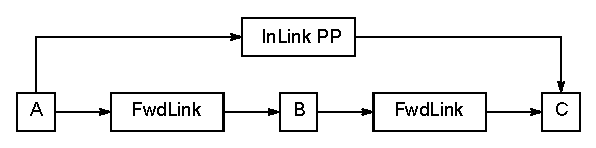
\includegraphics{lockScanProcess_6}
\end{center}

Assume that A, B, and C are all passive records. The notation states that A has a forward link to B and B to C. C has an 
input link obtaining a value from A. Assume, for some reason, A gets processed. The following sequence of events 
occurs:

\begin{enumerate}
\item A begins processing. While processing a request is made to process B.

\item B starts processing. While processing a request is made to process C.

\item C starts processing. One of the first steps is to get a value from A via the input link.

\item At this point a question occurs. Note that the input link specifies process passive (signified by the \verb|PP| after 
\verb|InLink|). But process passive states that A should be processed before the value is retrieved. Are we in an infinite 
loop? The answer is no. Every record contains a field \verb|pact| (processing active), which is set \verb|TRUE| when record 
processing begins and is not set \verb|FALSE| until all processing completes. When C is processed A still has \verb|pact| \verb|TRUE| 
and will not be processed again.

\item C obtains the value from A and completes its processing. Control returns to B.

\item B completes returning control to A

\item A completes processing.

\end{enumerate}

This brief example demonstrates that database links needs more discussion.

\subsection{Rules Relating to Database Links}

\subsubsection{Processing Order}

The processing order is guaranteed to follow the following rules:

\begin{enumerate}
\item Forward links are processed in order from left to right and top to bottom. For example the following records are 
processed in the order \verb|FLNK1|, \verb|FLNK2|, \verb|FLNK3|, \verb|FLNK4| .

\begin{center}
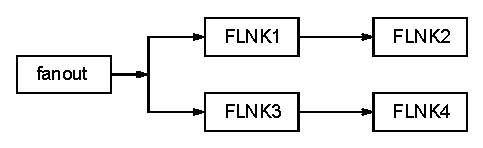
\includegraphics{lockScanProcess_9}
\end{center}

\item If a record has multiple input links (calculation and select records) the input is obtained in the natural order. For 
example if the fields are named \verb|INPA|, \verb|INPB|, ..., \verb|INPL|, then the links are read in the order A then B then C, etc. 
Thus if obtaining an input results in a record being processed, the processing order is guaranteed.

\item All input and output links are processed before the forward link.

\end{enumerate}

\subsubsection{Lock Sets}

All records, except for the conditions listed in the next paragraph, linked together directly or indirectly are placed in the 
same lock set. When \verb|dbScanLock| is called the entire set, not just the specified record, is locked. This prevents two 
different tasks from simultaneously modifying records in the same lock set.

\subsubsection{PACT - processing active}

Each record contains a field \verb|pact|. This field is set \verb|TRUE| at the beginning of record processing and is not set \verb|FALSE| until 
the record is completely processed. In particular no links are processed with \verb|pact| \verb|FALSE|. This prevents infinite 
processing loops. The example given at the beginning of this section gives an example. It will be seen in the next two 
sections that \verb|pact| has other uses.

\subsubsection{Process Passive: Link option}

Input and output links have an option called process passive. For each such link the application developer can specify 
process passive \verb|TRUE| (\verb|PP|) or process passive \verb|FALSE| (\verb|NPP|). Consider the following example 

\begin{center}
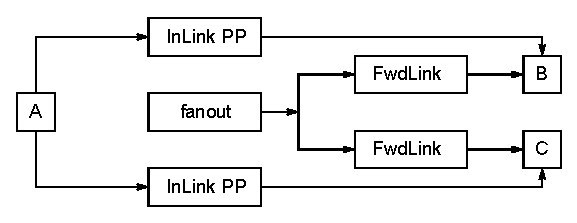
\includegraphics{lockScanProcess_16}
\end{center}

Assume that all records except fanout are passive. When the fanout record is processed the following sequence of events 
occur:

\begin{enumerate}
\item Fanout starts processing and asks that B be processed.

\item B begins processing. It calls \verb|dbGetLink| to obtain data from A.

\item Because the input link has process passive true, a request is made to process A.

\item A is processed, the data value fetched, and control is returned to B

\item B completes processing and control is returned to fanout. Fanout asks that C be processed.

\item C begins processing. It calls \verb|dbGetLink| to obtain data from A.

\item Because the input link has process passive \verb|TRUE|, a request is made to process A.

\item A is processed, the data value fetched, and control is returned to C.

\item C completes processing and returns to fanout

\item The fanout completes

\end{enumerate}

Note that A got processed twice. This is unnecessary. If the input link to C is declared no process passive then A will only 
be processed once. Thus we should have .

\begin{center}
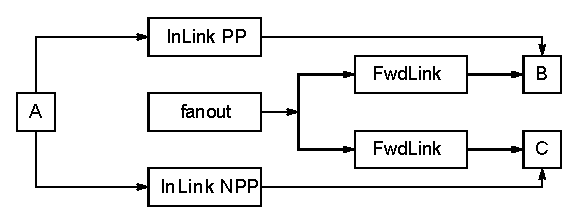
\includegraphics{lockScanProcess_26}
\end{center}

\subsubsection{Process Passive: Field attribute }

Each field of each database record type has an attribute called \verb|process_passive|. This attribute is specified in the  
record definition file. It is not under the control of the application developer. This attribute is used only by \verb|dbPutField|. 
It determines if a passive record will be processed after \verb|dbPutField| changes a field in the record. Consult the record 
specific information in the record reference manual for the setting of individual fields.

\subsubsection{Maximize Severity: Link option}

Input and output links have an option called maximize severity. For each such link the application developer can specify 
maximize severity \verb|TRUE| (\verb|MS|) or maximize severity \verb|FALSE| (\verb|NMS|). 

When database input or output links are defined, the application developer can specify if alarm severities should be 
propagated across links. For input links the severity is propagated from the record referred to by the link to the record 
containing the link. For output links the severity of the record containing the link is propagated to the record referenced by 
the link. The alarm severity is transferred only if the new severity will be greater than the current severity. If the severity 
is propagated the alarm status is set equal to \verb|LINK_ALARM|.

\section{Guidelines for Synchronous Records}

\index{Guidelines for Synchronous Records}
A synchronous record is a record that can be completely processed without waiting. Thus the application developer never 
needs to consider the possibility of delays when he defines a set of related records. The only consideration is deciding 
when records should be processed and in what order a set of records should be processed.

The following reviews the methods available to the application programmer for deciding when to process a record and for 
enforcing the order of record processing.

\begin{enumerate}
\item A record can be scanned periodically (at one of several rates), via I/O event, or via Event.

\item For each periodic group and for each Event group the phase field can be used to specify processing order.

\item The application programmer has no control over the record processing order of records in different groups.

\item The disable fields (\verb|SDIS|, \verb|DISA|, and \verb|DISV|) can be used to disable records from being processed. By letting the 
\verb|SDIS| field of an entire set of records refer to the same input record, the entire set can be enabled or disabled 
simultaneously. See the Record Reference Manual for details.

\item A record (periodic or other) can be the root of a set of passive records that will all be processed whenever the root 
record is processed. The set is formed by input, output, and forward links.

\item The \verb|process_passive| option specified for each field of each record determines if a passive record is processed 
when a \verb|dbPutField| is directed to the field. The application developer must be aware of the possibility of record 
processing being triggered by external sources if \verb|dbPutFields| are directed to fields that have 
\verb|process_passive| \verb|TRUE|.

\item The \verb|process_passive| option for input and output links provides the application developer control over how a 
set of records are scanned.

\item General link structures can be defined. The application programmer should be wary, however, of defining arbitrary 
structures without carefully analyzing the processing order. 

\end{enumerate}

\section{Guidelines for Asynchronous Records}

\index{Guidelines for Asynchronous Records}
The previous discussion does not allow for asynchronous records. An example is a GPIB input record. When the record is 
processed the GPIB request is started and the processing routine returns. Processing, however, is not really complete until 
the GPIB request completes. This is handled via an asynchronous completion routine. Lets state a few attributes of 
asynchronous record processing. 

During the initial processing for all asynchronous records the following is done:

\begin{enumerate}
\item \verb|pact| is set \verb|TRUE|

\item Data is obtained for all input links

\item Record processing is started

\item The record processing routine returns

\end{enumerate}

The asynchronous completion routine performs the following algorithm:

\begin{enumerate}
\item Record processing continues

\item Record specific alarm conditions are checked

\item Monitors are raised

\item Forward links are processed

\item \verb|pact| is set \verb|FALSE|.

\end{enumerate}

A few attributes of the above rules are:

\begin{enumerate}
\item Asynchronous record processing does not delay the scanners.

\item Between the time record processing begins and the asynchronous completion routine completes, no attempt will be 
made to again process the record. This is because \verb|pact| is \verb|TRUE|. The routine \verb|dbProcess| checks \verb|pact| and does 
not call the record processing routine if it is \verb|TRUE|. Note, however, that if \verb|dbProcess| finds the record active 10 
times in succession, it raises a \verb|SCAN_ALARM|.

\item Forward and output links are triggered only when the asynchronous completion routine completes record 
processing.

\end{enumerate}

With these rules the following works just fine:

\begin{center}
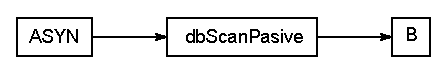
\includegraphics{lockScanProcess_34}
\end{center}

When \verb|dbProcess| is called for record ASYN, processing will be started but \verb|dbScanPassive| will not be called. Until 
the asynchronous completion routine executes any additional attempts to process ASYN are ignored. When the 
asynchronous callback is invoked the \verb|dbScanPassive| is performed.

Problems still remain. A few examples are:

\subsection{Infinite Loop}

\index{Infinite Loop}
Infinite processing loops are possible.

\begin{center}
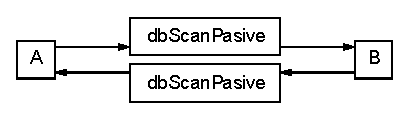
\includegraphics{lockScanProcess_1}
\end{center}

Assume both A and B are asynchronous passive records and a request is made to process A. The following sequence of 
events occur.

\begin{enumerate}
\item A starts record processing and returns leaving \verb|pact| \verb|TRUE|.

\item Sometime later the record completion for A occurs. During record completion a request is made to process B. B 
starts processing and control returns to A which completes leaving its \verb|pact| field \verb|FALSE|.

\item Sometime later the record completion for B occurs. During record completion a request is made to process A. A 
starts processing and control returns to B which completes leaving its \verb|pact| field \verb|FALSE|.

\end{enumerate}

Thus an infinite loop of record processing has been set up. It is up to the application developer to prevent such loops.

\subsection{Obtain Old Data}

A \verb|dbGetLink| to a passive asynchronous record can get old data.

\begin{center}

\includegraphics{lockScanProcess_37}
\end{center}

If A is a passive asynchronous record then the \verb|dbGetLink| request forces \verb|dbProcess| to be called for A. \verb|dbProcess| 
starts the processing and returns. \verb|dbGetLink| then reads the desired value which is still old because processing will only 
be completed at a later time.

\subsection{Delays}

Consider the following:

\begin{center}
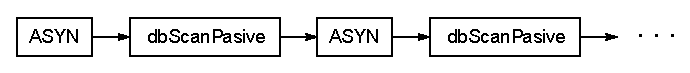
\includegraphics{lockScanProcess_40}
\end{center}

The second ASYN record will not begin processing until the first completes, etc. This is not really a problem except that 
the application developer must be aware of delays caused by asynchronous records. Again, note that scanners are not 
delayed, only records downstream of asynchronous records. 

\subsection{Task Abort}

If the processing task aborts and the watch dog task cleans up before the asynchronous processing routine completes what 
happens? If the asynchronous routine completes before the watch dog task runs everything is okay. If it doesn't? This is a 
more general question of the consequences of having the watchdog timer restart a scan task. EPICS currently does not 
allow scanners to be automatically restarted. 

\section{Cached Puts}

\index{Cached Puts}
The rules followed by \verb|dbPutLink| and \verb|dbPutField| provide for ``cached" puts. This is necessary because of 
asynchronous records. Two cases arise.

The first results from a \verb|dbPutField|, which is a put coming from outside the database, i.e. Channel Access puts. If this 
is directed to a record that already has \verb|pact| \verb|TRUE| because the record started processing but asynchronous completion 
has not yet occurred, then a value is written to the record but nothing will be done with the value until the record is again 
processed. In order to make this happen \verb|dbPutField| arranges to have the record reprocessed when the record finally 
completes processing.

The second case results from \verb|dbPutLink| finding a record already active because of a \verb|dbPutField| directed to the 
record. In this case \verb|dbPutLink| arranges to have the record reprocessed when the record finally completes processing. If 
the record is already active because it appears twice in a chain of record processing, it is not reprocessed because the chain 
of record processing would constitute an infinite loop.

Note that the term caching not queuing is used. If multiple requests are directed to a record while it is active, each new 
value is placed in the record but it will still only be processed once, i.e. last value wins.

\section{putNotify}

\index{putNotify}
\index{dbPutNotify}dbPutNotify, which is called when a Channel Access client calls \index{ca\_put\_callback}ca\_put\_callback, is a request to notify the caller when all 
records processed as a result of the put complete. Because of asynchronous records this can be complicated and the set of 
records that are processed because of a put may not be deterministic. The result of a dbPutNotify is the same as a 
dbPutField except for the following:

\begin{itemize}
\item dbPutNotifys are queued rather than cached. Thus when additional dbPutNotifys are directed to a record that 
already has an active dbPutNotify, they are queued. As each one finishes it releases the next one in the queue.

\item If a dbPutNotify links to a record that is not active but has a dbPutNotify attached to it, no attempt is made to 
process the record.

\end{itemize}

\section{Channel Access Links}

A channel access link is:

\begin{enumerate}
\item A record link that references a record in a different IOC.

\item A link that the application developer forces to be a channel access link.

\end{enumerate}

A channel access client task (dbCa)  handles all I/O for channel access links. It does the following:

\begin{itemize}
\item At IOC initialization dbCa issues channel access search requests for each channel access link.

\item For each input link it establishes a channel access monitor. It uses \verb|ca_field_type| and \verb|ca_element_count| 
when it establishes the monitor. It also monitors the alarm status. Whenever the monitor is invoked the new data is 
stored in a buffer belonging to dbCa. When iocCore or the record support module asks for data the data is taken 
from the buffer and converted to the requested type.

\item For each output link, a buffer is allocated the first time iocCore/record support issues a put and a channel access 
connection has been made. This buffer is allocated according to  \verb|ca_field_type| and \verb|ca_element_count|. 
Each time iocCore/record support issues a put, the data is converted and placed in the buffer and a request is made 
to dbCa to issue a new ca\_put.

\end{itemize}

Even if a link references a record in the same IOC it can be useful to force it to act like a channel access link. In particular 
the records will not be forced to be in the same lock set. As an example consider a scan record that links to a set of 
unrelated records, each of which can cause a lot of records to be processed. It is often NOT desirable to force all these 
records into the same lock set. Forcing the links to be handled as channel access links solves the problem.

CA links which connect between IOCs incur the extra overhead associated with message passing protocols, operating 
system calls, and network activity. In contrast, CA links which connect records in the same IOC are executed more 
efficiently by directly calling database access functions such as dbPutField() and dbGetField(), or by receiving callbacks 
directly from a database monitor subscription event queue.

Because channel access links interact with the database only via dbPutField, dbGetField, and a database monitor 
subscription event queue, their interaction with the database is fundamentally different from database links which are 
tightly integrated within the code that executes database records. For this reason and because channel access does not 
understand process passive or maximize severity, the semantics of channel access links are not the same as database links. 
Let's discuss the channel access semantics of INLINK, OUTLINK, and FWDLINK separately.

\subsection{INLINK}

The options for process passive are:

\begin{itemize}
\item PP or NPP - This link is made a channel access link because the referenced record is not found in the local IOC. It 
is not possible to honor PP, thus the link always acts like NPP.

\item CA - Force the link to be a channel access link.

\item CP - Force the link to be a channel access link and also request that the record containing the link be processed 
whenever a monitor occurs.

\item CPP - Force the link to be a channel access link and also request that the record containing the link, if it is passive, 
be processed whenever a monitor occurs.

\end{itemize}

Maximize Severity is honored.

\subsection{OUTLINK}

The options for process passive are:

\begin{itemize}
\item PP or NPP - This link is made a channel access link because the referenced record is not found in the local IOC. It 
is not possible to honor PP thus the link always acts like NPP.

\item CA - Force the link to be a channel access link.

\end{itemize}

Maximize Severity is not honored.

\subsection{FWDLINK}

A channel access forward link is honored only if it references the PROC field of a record. In that case a ca\_put with a 
value of 1 is written each time a forward link request is issued.

The options for process passive are:

\begin{itemize}
\item PP or NPP - This link is made a channel access link because the referenced record is not found in the local IOC. It 
is not possible to honor PP thus it always acts like NPP.

\item CA - Force the link to be a channel access link.

\end{itemize}

Maximize Severity is not honored.


